\documentclass[11pt,letterpaper]{article}
\usepackage[margin=0.68in,headheight=16pt,headsep=18pt,footskip=25pt]{geometry}
\usepackage[T1]{fontenc}
\usepackage{lmodern}
\renewcommand{\familydefault}{\sfdefault}
\usepackage{microtype,amsmath,amssymb,array,tabularx,booktabs}
\usepackage[table]{xcolor}
\usepackage{tikz}
\usetikzlibrary{arrows.meta,positioning,calc,shapes.geometric}
\usepackage[most]{tcolorbox}
\usepackage{enumitem,fancyhdr,hyperref}
\hypersetup{colorlinks=true,urlcolor=teal,linkcolor=teal,pdftitle={ClearView: A Visual Project Explainer},pdfauthor={TAPIA Hackathon Project Planning}}
\definecolor{navy}{HTML}{142D42}
\definecolor{teal}{HTML}{007F79}
\definecolor{mint}{HTML}{E8F5F2}
\definecolor{amber}{HTML}{A45A06}
\definecolor{sand}{HTML}{FFF3DF}
\definecolor{red}{HTML}{B44144}
\definecolor{rose}{HTML}{FBECEE}
\definecolor{ink}{HTML}{243A4A}
\definecolor{muted}{HTML}{5D7180}
\definecolor{line}{HTML}{D9E3E9}
\definecolor{pale}{HTML}{F2F6F8}
\color{ink}
\setlength{\parindent}{0pt}
\setlength{\parskip}{7pt}
\setlength{\tabcolsep}{7pt}
\renewcommand{\arraystretch}{1.25}
\setlist[itemize]{leftmargin=16pt,itemsep=3pt,topsep=3pt}
\pagestyle{fancy}
\fancyhf{}
\fancyhead[L]{\small\bfseries\color{teal} CLEARVIEW}
\fancyhead[R]{\small\color{muted} TAPIA 2026 / CHALLENGE 09}
\fancyfoot[L]{\footnotesize\color{muted} Proposed design \textbullet\ Visual explainer}
\fancyfoot[R]{\footnotesize\color{muted}\thepage\ / 4}
\renewcommand{\headrulewidth}{0.4pt}
\renewcommand{\footrulewidth}{0pt}
\newcommand{\eyebrow}[1]{{\small\bfseries\color{teal}#1}\par\vspace{3pt}}
\newcommand{\pagetitle}[2]{{\fontsize{27}{30}\selectfont\bfseries\color{navy}#1}\par\vspace{4pt}{\large\color{muted}#2}\par\vspace{9pt}}
\newcommand{\sect}[1]{\vspace{6pt}{\large\bfseries\color{navy}#1}\par\vspace{2pt}}
\newcommand{\smallnote}[1]{{\footnotesize\color{muted}#1}\par}
\newtcolorbox{card}[2][]{enhanced,boxrule=0pt,arc=3mm,colback=pale,colframe=line,left=12pt,right=12pt,top=10pt,bottom=10pt,title={#2},coltitle=navy,fonttitle=\bfseries,colbacktitle=pale,attach title to upper={\par\smallskip},#1}
\tikzset{arr/.style={-{Stealth[length=2.5mm]},line width=1.1pt,draw=teal},
  box/.style={rounded corners=3mm,draw=line,fill=pale,align=left,inner sep=10pt,font=\small,text=ink},
  agentstep/.style={box,text width=4.0cm,minimum height=1.6cm}}
\begin{document}

\eyebrow{01 / THE BIG PICTURE}
\pagetitle{What are we building?}{An AI data detective that must justify every repair.}

Imagine a spreadsheet with repeated sales, missing quantities, and strange values.
ClearView investigates the problems, repairs what the evidence supports,
and asks a person about anything ambiguous.

\begin{center}
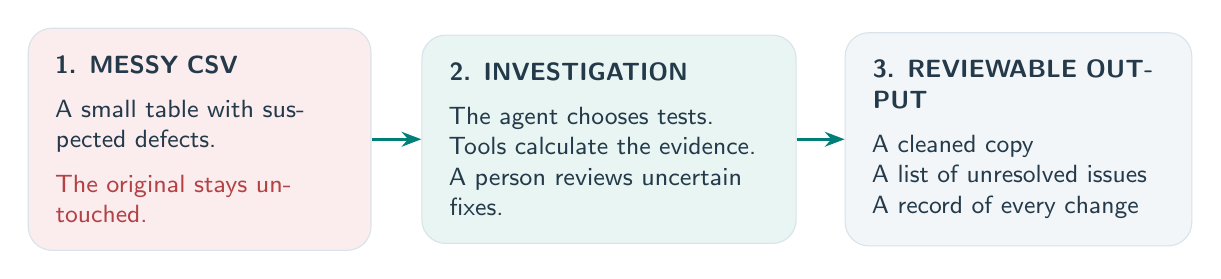
\begin{tikzpicture}
\node[box,fill=rose,text width=3.65cm,minimum height=2.25cm] (input) at (0,0) {\textbf{1. MESSY CSV}\\[5pt]A small table with suspected defects.\\[5pt]\textcolor{red}{The original stays untouched.}};
\node[box,fill=mint,text width=4.05cm,minimum height=2.25cm] (agent) at (5.2,0) {\textbf{2. INVESTIGATION}\\[5pt]The agent chooses tests.\\Tools calculate the evidence.\\A person reviews uncertain fixes.};
\node[box,fill=pale,text width=3.7cm,minimum height=2.25cm] (output) at (10.4,0) {\textbf{3. REVIEWABLE OUTPUT}\\[5pt]A cleaned copy\\A list of unresolved issues\\A record of every change};
\draw[arr] (input.east) -- (agent.west);
\draw[arr] (agent.east) -- (output.west);
\end{tikzpicture}
\end{center}

\sect{What makes it an agent?}
A fixed script follows the same recipe every time. Here, the agent chooses its next
test from what it finds. If the evidence is weak, it investigates further or asks a human.

\begin{center}
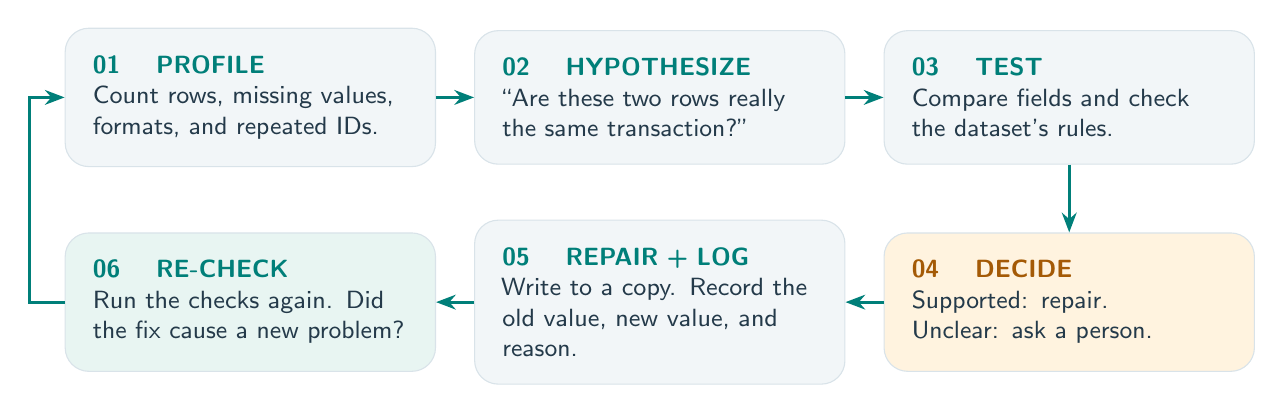
\begin{tikzpicture}
\node[agentstep] (profile) at (0,0) {\textcolor{teal}{\textbf{01 \quad PROFILE}}\\Count rows, missing values, formats, and repeated IDs.};
\node[agentstep] (hypothesis) at (5.2,0) {\textcolor{teal}{\textbf{02 \quad HYPOTHESIZE}}\\``Are these two rows really the same transaction?''};
\node[agentstep] (test) at (10.4,0) {\textcolor{teal}{\textbf{03 \quad TEST}}\\Compare fields and check the dataset's rules.};
\node[agentstep,fill=mint] (recheck) at (0,-2.6) {\textcolor{teal}{\textbf{06 \quad RE-CHECK}}\\Run the checks again. Did the fix cause a new problem?};
\node[agentstep] (repair) at (5.2,-2.6) {\textcolor{teal}{\textbf{05 \quad REPAIR + LOG}}\\Write to a copy. Record the old value, new value, and reason.};
\node[agentstep,fill=sand] (decide) at (10.4,-2.6) {\textcolor{amber}{\textbf{04 \quad DECIDE}}\\Supported: repair.\\Unclear: ask a person.};
\draw[arr] (profile) -- (hypothesis);
\draw[arr] (hypothesis) -- (test);
\draw[arr] (test) -- (decide);
\draw[arr] (decide) -- (repair);
\draw[arr] (repair) -- (recheck);
\draw[arr] (recheck.west) -- ++(-0.45,0) |- (profile.west);
\end{tikzpicture}
\end{center}

\begin{card}[colback=navy,colbacktitle=navy,coltitle=white,coltext=white]{The core promise}
Every repair has a reason you can inspect. A surprising value is a clue to investigate;
it is not, by itself, proof that the data is wrong.
\end{card}
\smallnote{Status: this document explains the proposed prototype. The product has not yet been built or evaluated.}

\newpage
\eyebrow{02 / A WORKED EXAMPLE}
\pagetitle{Watch one investigation}{Five cafe sales. Three decisions. Different kinds of evidence.}

\smallnote{Illustrative data only. The examples below are expected behavior, not results from a working system. All prices are in USD.}
\vspace{2pt}
\begin{tabularx}{\linewidth}{@{}l l X r r r@{}}
\toprule
\textbf{Row} & \textbf{Sale ID} & \textbf{Item} & \textbf{Qty.} & \textbf{Unit price} & \textbf{Total}\\
\midrule
1 & T101 & Coffee & 2 & 3.00 & 6.00\\
\rowcolor{rose}2 & T101 & Coffee & 2 & 3.00 & 6.00\\
\rowcolor{sand}3 & T102 & Tea & \textcolor{amber}{\textbf{?}} & 2.50 & 7.50\\
4 & T103 & Sandwich & 1 & 8.00 & 8.00\\
\rowcolor{mint}5 & T104 & Coffee & \textbf{20} & 3.00 & 60.00\\
\bottomrule
\end{tabularx}

\begin{card}[colback=pale]{The rules must be known first}
\small In this example, each Sale ID identifies exactly one sale row. Quantity is a
positive whole number, prices and totals are trusted, and there are no taxes,
discounts, or refunds. These are supplied data rules, not assumptions the AI may invent.
\end{card}

\begin{card}[colback=rose,colbacktitle=rose]{A / Two identical rows: a supported repair}
Rows 1 and 2 have the same ID \emph{and} matching fields. Under the unique-ID rule,
row 2 is an extra copy. Keep row 1; remove row 2 from the cleaned copy.

\textbf{Evidence:} identical record + a rule saying that ID must be unique.
If an ID can span several line items, this rule no longer justifies deletion.
\end{card}

\begin{card}[colback=sand,colbacktitle=sand]{B / Missing quantity: recover it from trusted fields}
For row 3, the known accounting rule gives:
\[
\text{quantity}=\frac{\text{total}}{\text{unit price}}
=\frac{7.50}{2.50}=3.
\]
Set the quantity to \textbf{3}; then verify that $3\times 2.50=7.50$.
Without the stated rules, this would be a proposal for review, not an automatic fix.
\end{card}

\begin{card}[colback=mint,colbacktitle=mint]{C / Twenty coffees: unusual does not mean incorrect}
Row 5 is large, but $20\times 3.00=60.00$ is consistent. It could be a group order.
\textbf{Keep 20 unchanged.} A person can check the receipt if clarification is needed.
The agent must not replace it with a typical value simply because it is unusual.
\end{card}

\vspace{3pt}
\begin{center}
\color{navy}\bfseries
Cleaned example: 4 rows \quad\textbullet\quad T102 quantity = 3
\quad\textbullet\quad T104 quantity stays 20
\end{center}
\smallnote{The change log records row 2's removal and row 3's replacement, with reasons. The original five-row file is preserved so each change can be undone.}

\newpage
\eyebrow{03 / WHAT YOU WOULD SEE}
\pagetitle{The investigation screen}{One place to see the issue, the evidence, and the proposed action.}

\begin{center}
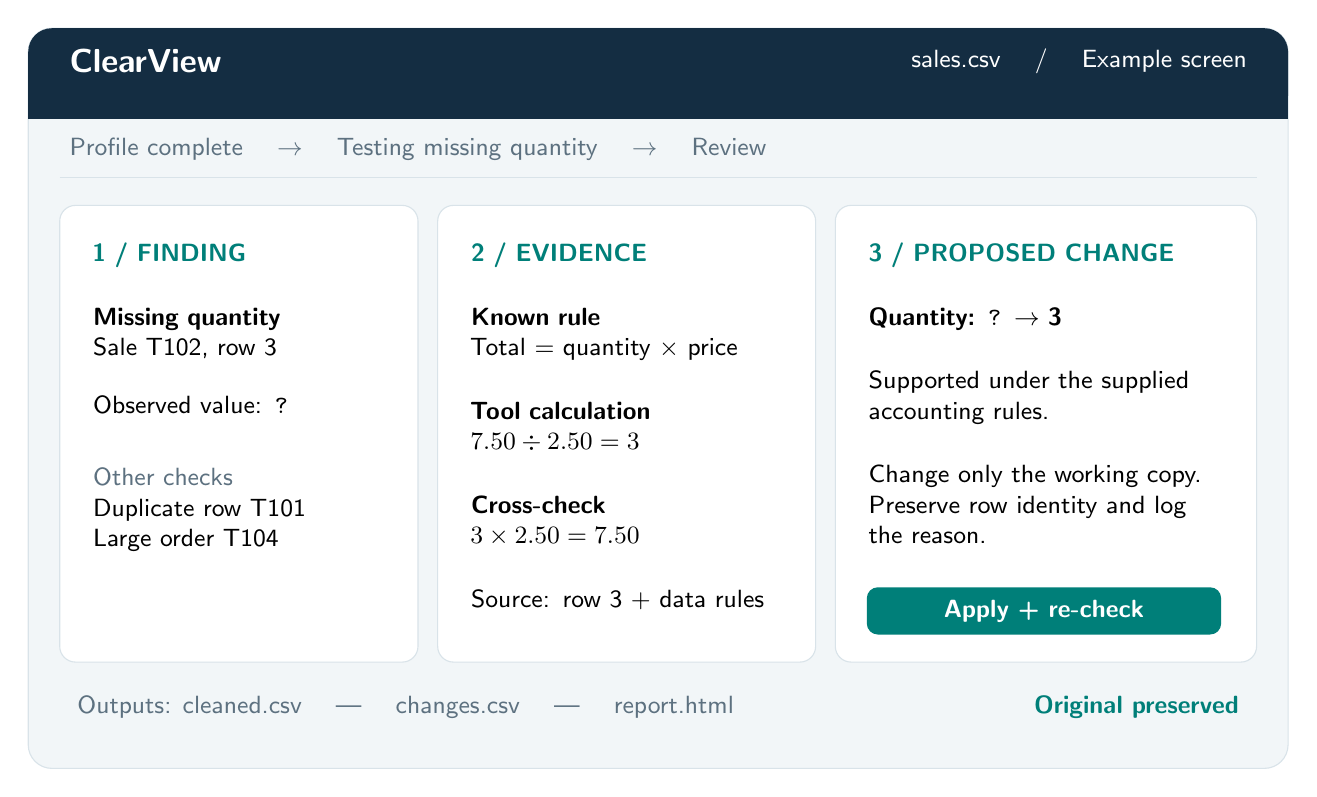
\begin{tikzpicture}[x=1cm,y=1cm]
\filldraw[fill=pale,draw=line,rounded corners=3mm] (0,0) rectangle (16,9.4);
\fill[navy,rounded corners=3mm] (0,8.25) rectangle (16,9.4);
\fill[navy] (0,8.25) rectangle (16,8.75);
\node[anchor=west,text=white,font=\large\bfseries] at (0.4,8.98) {ClearView};
\node[anchor=east,text=white,font=\small] at (15.6,8.98) {sales.csv \quad / \quad Example screen};
\node[anchor=west,text=muted,font=\small] at (0.4,7.86) {Profile complete \quad $\rightarrow$ \quad Testing missing quantity \quad $\rightarrow$ \quad Review};
\draw[line] (0.4,7.5) -- (15.6,7.5);
\filldraw[fill=white,draw=line,rounded corners=2mm] (0.4,1.35) rectangle (4.95,7.15);
\filldraw[fill=white,draw=line,rounded corners=2mm] (5.2,1.35) rectangle (10.0,7.15);
\filldraw[fill=white,draw=line,rounded corners=2mm] (10.25,1.35) rectangle (15.6,7.15);
\node[anchor=north west,text width=3.85cm,font=\small,align=left] at (0.7,6.8) {\textcolor{teal}{\textbf{1 / FINDING}}\\[12pt]\textbf{Missing quantity}\\Sale T102, row 3\\[10pt]Observed value: \texttt{?}\\[15pt]\textcolor{muted}{Other checks}\\Duplicate row T101\\Large order T104};
\node[anchor=north west,text width=4.05cm,font=\small,align=left] at (5.5,6.8) {\textcolor{teal}{\textbf{2 / EVIDENCE}}\\[12pt]\textbf{Known rule}\\Total = quantity $\times$ price\\[12pt]\textbf{Tool calculation}\\$7.50\div 2.50=3$\\[12pt]\textbf{Cross-check}\\$3\times 2.50=7.50$\\[12pt]Source: row 3 + data rules};
\node[anchor=north west,text width=4.5cm,font=\small,align=left] at (10.55,6.8) {\textcolor{teal}{\textbf{3 / PROPOSED CHANGE}}\\[12pt]\textbf{Quantity: \texttt{?} $\rightarrow$ 3}\\[12pt]Supported under the supplied accounting rules.\\[12pt]Change only the working copy. Preserve row identity and log the reason.};
\fill[teal,rounded corners=1.4mm] (10.65,1.7) rectangle (15.15,2.3);
\node[text=white,font=\small\bfseries] at (12.9,2.0) {Apply + re-check};
\node[anchor=west,text=muted,font=\small] at (0.5,0.78) {Outputs: cleaned.csv \quad | \quad changes.csv \quad | \quad report.html};
\node[anchor=east,text=teal,font=\small\bfseries] at (15.5,0.78) {Original preserved};
\end{tikzpicture}
\end{center}
\smallnote{Design mockup, not an application screenshot. An ambiguous case would show a human-review action instead of an automatic repair. No invented accuracy or confidence percentages.}

\sect{Who does what?}
\begin{minipage}[t]{0.485\linewidth}
\vspace{0pt}
\begin{card}[colback=mint,colbacktitle=mint,height=3.5cm]{The agent and its tools}
\small
\textbf{Agent:} chooses what to investigate, selects a tool, interprets the result,
and chooses repair, more testing, or review.

\textbf{Tools:} count, compare, calculate, apply a patch to a copy, and run checks again.
\end{card}
\end{minipage}\hfill
\begin{minipage}[t]{0.485\linewidth}
\vspace{0pt}
\begin{card}[colback=sand,colbacktitle=sand,height=3.5cm]{The human teammate}
\small
Supplies trustworthy data rules, resolves ambiguous cases, and checks the result
against the original source.

Can reject a proposed repair and explain why. A second AI agreeing is not a human check.
\end{card}
\end{minipage}

\newpage
\eyebrow{04 / HOW WE PROVE IT WORKS}
\pagetitle{The reveal is the demo}{Humans know the planted errors. The agent does not.}

\begin{center}
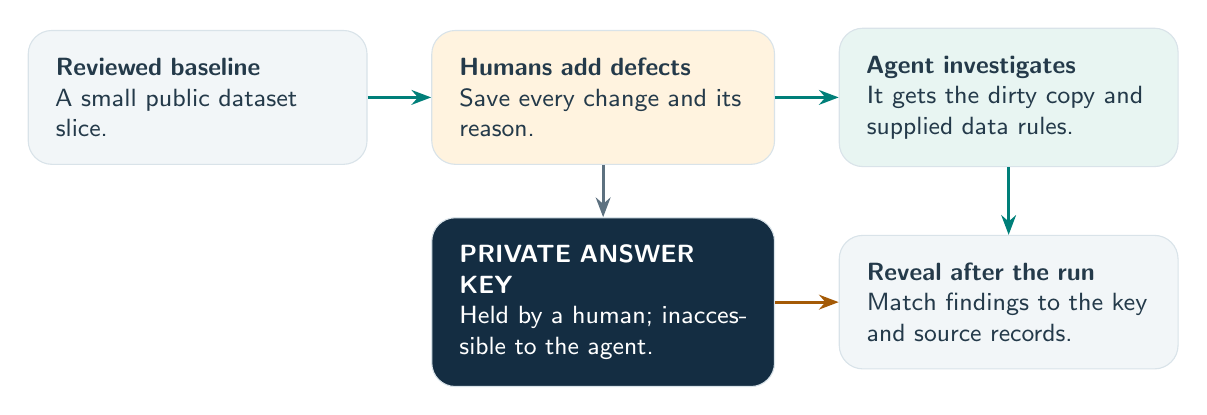
\begin{tikzpicture}
\node[box,text width=3.6cm,minimum height=1.7cm] (source) at (0,0) {\textbf{Reviewed baseline}\\A small public dataset slice.};
\node[box,text width=3.65cm,minimum height=1.7cm,fill=sand] (inject) at (5.15,0) {\textbf{Humans add defects}\\Save every change and its reason.};
\node[box,text width=3.6cm,minimum height=1.7cm,fill=mint] (run) at (10.3,0) {\textbf{Agent investigates}\\It gets the dirty copy and supplied data rules.};
\node[box,text width=3.65cm,minimum height=1.3cm,fill=navy,text=white] (key) at (5.15,-2.6) {\textbf{PRIVATE ANSWER KEY}\\Held by a human; inaccessible to the agent.};
\node[box,text width=3.6cm,minimum height=1.3cm] (reveal) at (10.3,-2.6) {\textbf{Reveal after the run}\\Match findings to the key and source records.};
\draw[arr] (source) -- (inject);
\draw[arr] (inject) -- (run);
\draw[arr,draw=muted] (inject.south) -- (key.north);
\draw[arr] (run.south) -- (reveal.north);
\draw[arr,draw=amber] (key.east) -- (reveal.west);
\end{tikzpicture}
\end{center}

\begin{tabularx}{\linewidth}{@{}>{\bfseries}l X@{}}
\toprule
\textcolor{teal}{CAUGHT} & A real defect was identified. Check repair correctness separately.\\
\textcolor{amber}{MISSED} & A real defect was not identified. Track unresolved repairs separately.\\
\textcolor{red}{FALSELY FLAGGED} & A valid value was incorrectly called an error; a human checks it.\\
\bottomrule
\end{tabularx}
\smallnote{Humans hold both the baseline and key until the agent's findings are frozen. Score only verified cases; the key does not prove that all other data is flawless. Show an actual agent mistake, never a fabricated one.}

\sect{A two-minute presentation}
\begin{tabularx}{\linewidth}{@{}>{\bfseries\color{teal}}p{2.15cm}X@{}}
0:00--0:20 & Show the messy file and explain the hidden answer key.\\
0:20--0:55 & Give one audit goal. Show the agent choosing and running tests.\\
0:55--1:20 & Open one finding; inspect the evidence and the actual repair.\\
1:20--1:45 & Reveal caught, missed, and falsely flagged cases. Explain a real human correction.\\
1:45--2:00 & Export the cleaned copy and change ledger. Show what remains unresolved.\\
\end{tabularx}

\sect{Keep the four-hour build small}
\begin{center}

\begin{tikzpicture}[x=0.063cm,y=1cm]
\foreach \a/\b/\c/\lab in {0/30/navy/Setup,30/90/teal/Agent loop,90/150/navy/Visual interface,150/195/teal/Human checks,195/240/navy/Rehearse}{
\fill[\c] (\a,0) rectangle (\b,0.6);
\node[font=\scriptsize,text=white] at ({(\a+\b)/2},0.3) {\lab};
}
\foreach \v in {0,30,90,150,195,240}{\node[anchor=north,font=\scriptsize,text=muted] at (\v,-0.08) {\v};}
\end{tikzpicture}
\end{center}
\smallnote{Estimated minutes, not a measured schedule. Setup includes verifying the model/tool connection and preparing a reviewed baseline.}

\textbf{MVP boundary:} one CSV, five defect types, a small tool set, one review screen,
and three export files. Start with duplicates and missing values; add invalid dates,
inconsistent labels, and documented unit mismatches. Keep a valid outlier as a control.

\vfill
\smallnote{Source: \textit{2026 - Hackathon Challenge Problems.pdf}, challenge 9, page 7. The challenge requires profile/check/fix/re-profile, reasons for fixes, and human verification. The interface, example data, and schedule in this explainer are proposed designs.}
\end{document}
